\begin{frame}
\begin{definition}[Campo Vectorial]
  Un \textbf{campo vectorial} $X$ en una variedad $M$ es una sección del fibrado tangente $\pi: TM \to M$, esto es, $X: M \to TM$ es un mapa tal que $X(p) \in T_{p}(M)$ para cada $p \in M$. Además diremos que que es un \textbf{campo vectorial suave} si $X$ es un mapa suave. Denotaremos al conjunto formado por todas los campos vectoriales suaves en $M$ como $\mathfrak{X}(M)$
\end{definition}
\end{frame}

\begin{frame}
  \centering
  \begin{figure}
  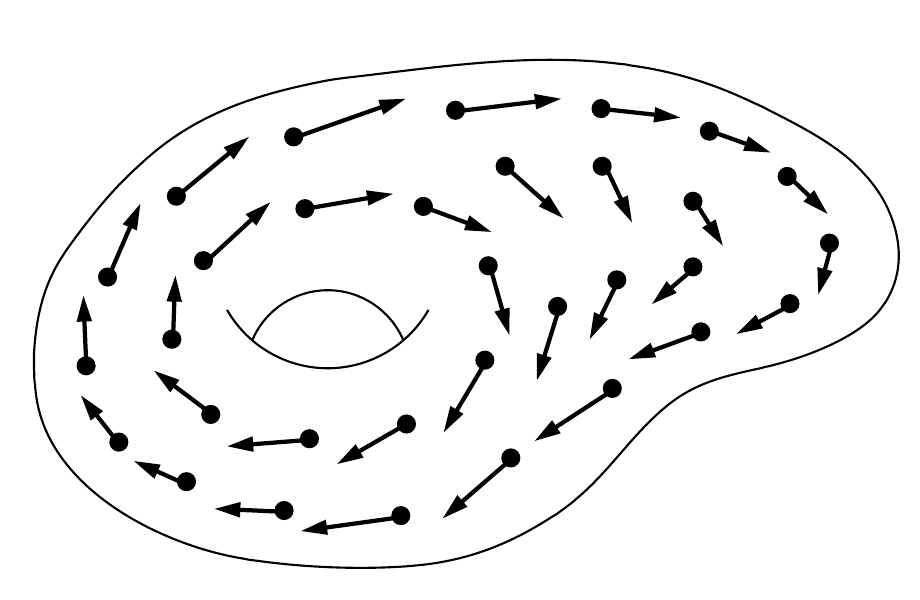
\includegraphics[width=0.8\textwidth]{./Figuras/CampoVectorial.png}
    \caption{Representación de un campo vectorial.}
  \end{figure}
\end{frame}
